\section{Functional role of classes}
\label{sec:functional-role}

\subsection{Java Transaction Service}
All the classes to review are part of the Java Transaction Service (JTS) implementation by Sun.

The complete specification of Java Transaction Service is available on Oracle's website~\cite{jts-specification} and defines JTS as follows:
\begin{quotation}
This is the Java Transaction Service (JTS) Specification.
JTS specifies the
implementation of a transaction manager which supports the JTA specification at
the high-level and implements the Java mapping of the OMG Object Transaction
Service (OTS) 1.1 Specification at the low-level.

JTS uses the CORBA OTS interfaces for interoperability and portability (that is, \textbf{CosTransactions} and CosTSPortability).
These interfaces define a standard mechanism for any implementation that utilizes IIOP (Internet InterORB Protocol) to generate and
propagate transaction context between JTS Transaction Managers. Note, this also
permits the use of other API over the IIOP transport mechanism to be used; for
example, RMI over IIOP is allowed.
\end{quotation}

The Wikipedia page about the Java Transaction Service\footnote{\url{https://en.wikipedia.org/wiki/Java_transaction_service}} also gives us some useful information:
\begin{quote}
The \textbf{Java Transaction Service (JTS)} is a specification for building a transaction manager that maps onto the Object Management Group (OMG) Object Transaction Service (OTS) used in the Common Object Request Broker Architecture (CORBA) architecture. It uses General Inter-ORB Protocol (IIOP) to propagate the transactions between multiple JTS transaction managers.
\end{quote}

Summing up, we are analyzing Sun's implementation of the JTS specification, which is the Java mapping of the CORBA Object Transaction Service Specification~\cite{omg-ots}.

\begin{figure}
\centering
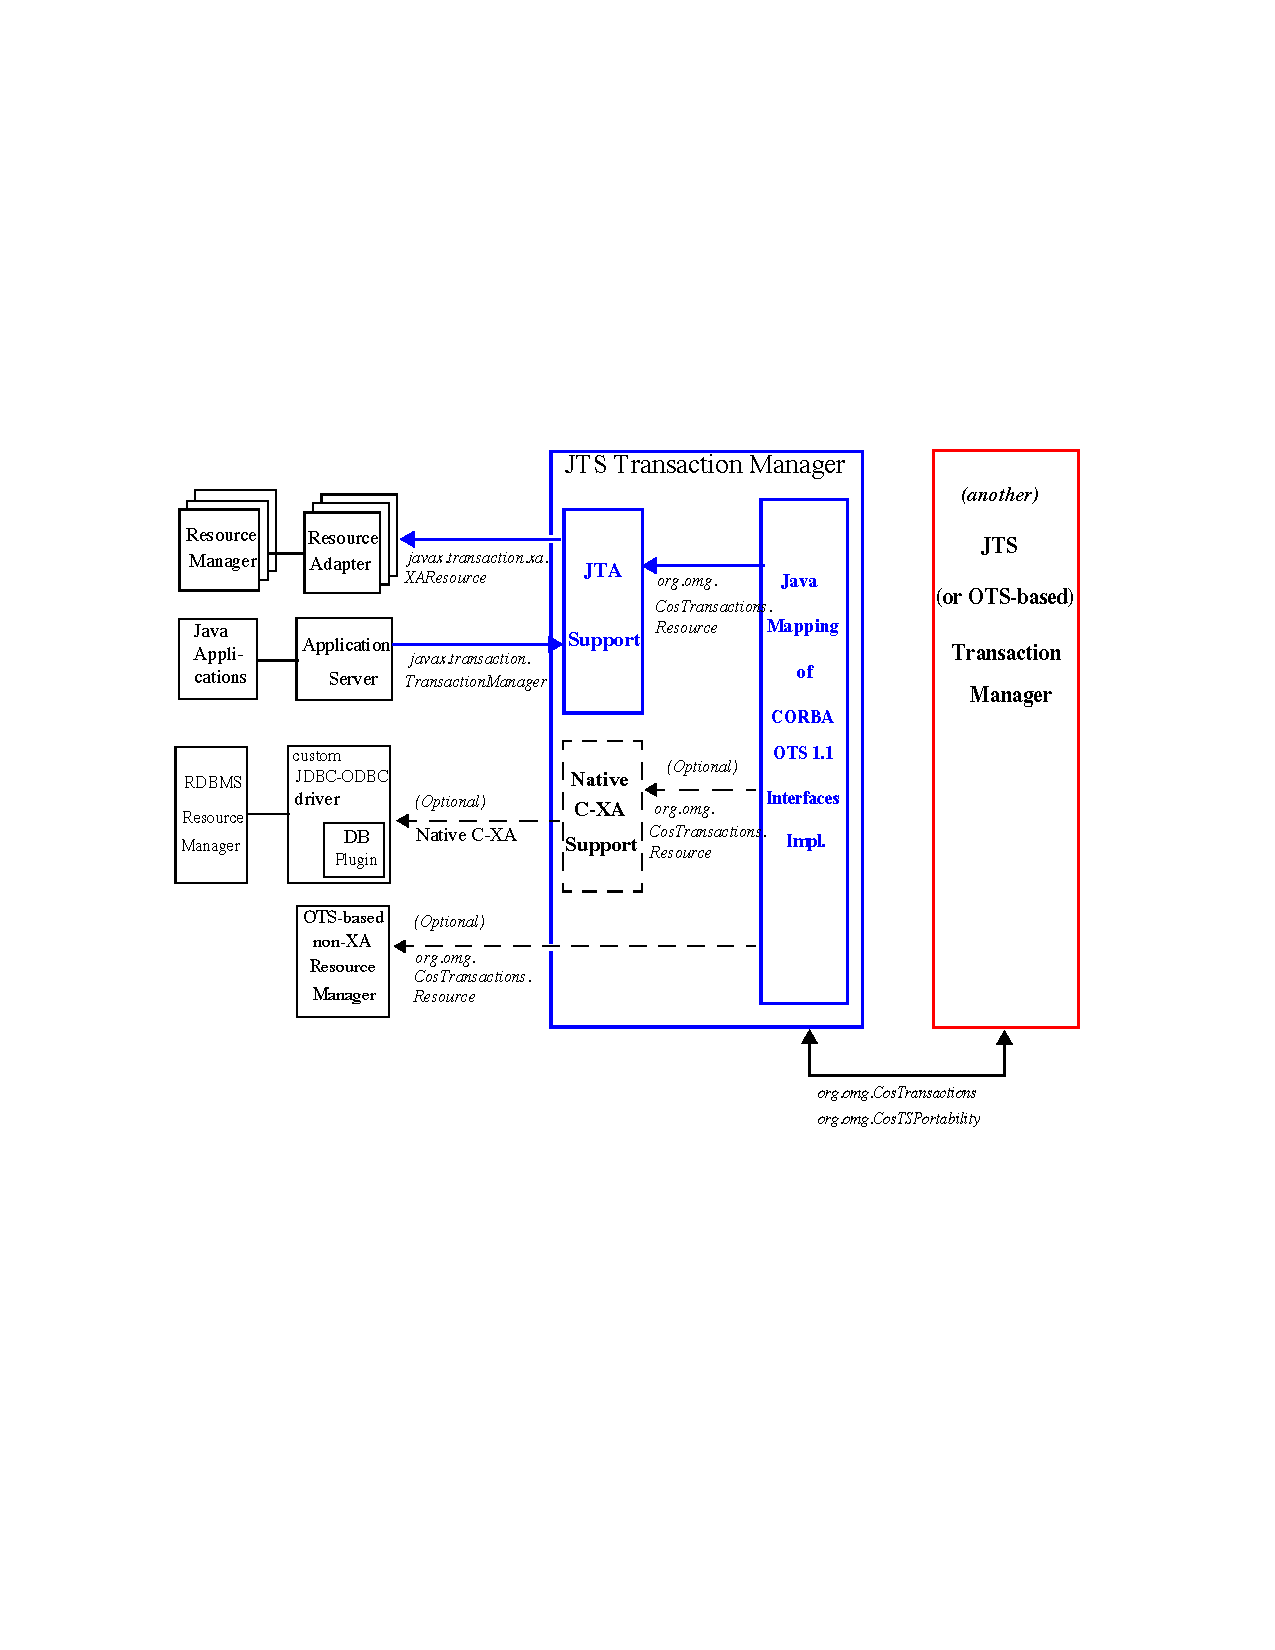
\includegraphics[width=0.8\textwidth]{figures/JTSDiagram}
\caption{This figure is taken from the JTS specification and shows the implementation of a JTS Transaction Manager.}
\label{fig:jts-diagram}
\end{figure}

The JTS specification also provides a component-like diagram (\autoref{fig:jts-diagram}) describing the structure of a possible implementation of a Transaction Manager.

\subsection{CosTransactions package}
The CosTransactions package is the Java implementation of the CosTransactions component, which is defined in the Transaction Service Specification of the Object Management Group~\cite{omg-ots}.

The particular subset of classes assigned to us implement part of the \emph{Reliability control system}~\cite[p.~311]{ceri-dbbook} of the transaction manager.
It ensures consistency and durability of the data in case of failure.

\subsection{CoordinatorLog class}
The CoordinatorLog class is contained in the CosTransactions package and is package-private. From the JavaDoc for the class, \codeline{79}:
\begin{quote}
    The CoordinatorLog interface provides operations to record transaction-specific information that needs to be persistently stored at a particular point in time, and subsequently restored.
\end{quote}

The CoordinatorLog class keeps the \textbf{transaction log} and writes it to persistent storage when needed. The log is a fundamental component in transaction managers and database systems. The log and the recovery manager together ensure consistency (i.e. the data must not stay in an inconsistent state) and durability (i.e. the committed transactions' data must be preserved) especially in case of failures.
The log allows to determine which transactions ended with a commit, which ones aborted and which ones are still running.
Details about log structure and reliability management are well explained in database theory books (see for example~\cite{ceri-dbbook}).

CoordinatorLog implements the \emph{LogUpcallTarget} interface that resides in the same package and is also package-private. Its JavaDoc reads:
\begin{quote}
    The LogUpcallTarget interface provides an operation that the log will call in the event it goes short-on-storage. This class must be sub-classed in order to implement the method that will handle the situation.
\end{quote}
The LogUpcallTarget provides the signature for the \texttt{upcall()} method.

\subsection{CoordinatorLogSection class}
The CoordinatorLogSection class is contained in the CosTransactions package, is package-private and does not implement any interface.
This class stores the data about the section of a CoordinatorLog.
The CoordinatorLog keeps track of the sections through an Hashtable (\texttt{sectionMapping} attribute).
From the JavaDoc for the class:
\begin{quote}
The CoordinatorLogSection class stores information relevant to a section.
\end{quote}

\subsection{RecoveryManager class}
The RecoveryManager class is contained in the CosTransactions package, it is public and does not implement any interface. From the JavaDoc for the class, \codeline{85}:
\begin{quote}
    This class manages information required for recovery, and also general state regarding transactions in a process.
\end{quote}

This class may be the implementation of the \emph{RecoveryCoordinator} interface defined in the OMG OTS specification~\cite[p. 47]{omg-ots}.

The RecoveryManager class is the component responsible to ensure consistency and durability in case of a fault, just as in relational databases.
When the system restarts after a failure, the RecoveryManager redoes committed transactions and undoes uncommitted (or aborted) ones, like in the \emph{warm restart} protocol in database systems~\cite[p.~319]{ceri-dbbook}.
